%% 
%% File:    PResCnam-final.tex
%% Author:  Stefano Secci (stefano.secci@lecnam.net)
%% Adapté pour le projet CNAM
%% 

\documentclass[a4paper,12pt]{article}

\usepackage[francais]{babel}
\usepackage{fancyhdr}
\usepackage[utf8]{inputenc}
\usepackage[T1]{fontenc}
\usepackage{epsfig}
\usepackage{calc}
\usepackage{url}
\usepackage{boxedminipage}
\usepackage{graphicx}
\usepackage{hyperref}
\usepackage{listings}
\usepackage{xcolor}

\definecolor{codeborder}{RGB}{180,30,30}
\definecolor{codebg}{RGB}{255,248,248}
\definecolor{codecomment}{RGB}{90,90,90}
\definecolor{codestring}{RGB}{160,90,20}

\lstdefinestyle{annexecode}{
  basicstyle=\ttfamily\footnotesize,
  keywordstyle=\bfseries,
  commentstyle=\color{codecomment}\itshape,
  stringstyle=\color{codestring},
  breaklines=true,
  frame=single,
  rulecolor=\color{codeborder},
  backgroundcolor=\color{codebg},
  numbers=left,
  numberstyle=\tiny\color{codecomment},
  tabsize=4,
  showstringspaces=false,
  xleftmargin=6pt,
  xrightmargin=6pt,
  framexleftmargin=6pt,
  framexrightmargin=6pt
}

%%%%%%%%%%%%%%%%%%%%%%%%%%%%%%%%%%%%%%%%%%%%%%%%%%%%%%%%%%%
%% Définitions à personnaliser 

%%%% Indiquer le nom de l'encadrant ci-dessous:
\def\nomEncad{Y. ~Benchaïb} % 

%%%% Indiquer les noms des étudiants participant ci-dessous:
\def\nomEtudA{J.~Mootooveeren}
\def\nomEtudB{A.~Atmane}
\def\nomEtudC{A.~Landois}
\def\nomEtudD{J.~Montguillon}

%%%% Indiquer la référence (numero) et le nom du sujet ci-dessous:
\def\refProjet{2} 
\def\titreProjetCourt{Tetragon \& eBPF IDS}
\def\titreProjetLong{Observabilité et graphes de comportement avec Tetragon pour des attaques zero-day}

\def\typeDoc{Rapport Final}
 
%%%%%%%%%%%%%%%%%%%%%%%%%%%%%%%%%%%%%%%%%%%%%%%%%%%%%%%%%%%
%% Définitions à ne pas modifier
 
\setlength{\voffset}{-1in} 
\setlength{\topmargin}{15mm}         
\setlength{\headheight}{20mm}        
\setlength{\headsep}{10mm}            
\setlength{\textheight}{220mm}       
\setlength{\footskip}{12mm}          

\setlength{\hoffset}{-1in} 
\setlength{\oddsidemargin}{25mm}     
\setlength{\evensidemargin}{25mm}    
\setlength{\marginparwidth}{0mm}     
\setlength{\marginparsep}{0mm}       
\setlength{\textwidth}{160mm}        

\def\annee{2026} % 

\begin{document}
\selectlanguage{francais}

%%%%%%%%%%%%%%%%%%%%%%%%%%%%%%%%%%%%%%%%%%%%%%%%%%%%%%%%%%%
%% Définition des en-têtes et pied de pages
\pagestyle{fancyplain}
\lhead[\fancyplain{}{\texttt{Conservatoire national des arts et métiers}\\
          UE \textbf{USRS7N} Mars \annee \\ \nomEncad}]
      {\fancyplain{}{\textsc{Conservatoire national des arts et métiers}\\
          UE \textbf{USRS7N} Mars \annee \\ \nomEncad}}
\chead[\fancyplain{}{\textbf{Projet \refProjet\\\titreProjetCourt}}]
      {\fancyplain{}{\textbf{Projet \refProjet\\\titreProjetCourt}}}
\rhead[\fancyplain{}{\nomEtudA\\\nomEtudB\\\nomEtudC\\\nomEtudD}]
      {\fancyplain{}{\nomEtudA\\\nomEtudB\\\nomEtudC\\\nomEtudD}}
\lfoot[\fancyplain{}{\includegraphics[width=3cm]{logo-cnam.png}}]
      {\fancyplain{}{\includegraphics[width=3cm]{logo-cnam.png}}}
\cfoot[\fancyplain{}{\textbf{\thepage/\pageref{fin}}}]
      {\fancyplain{}{\textbf{\thepage/\pageref{fin}}}}
\rfoot[\fancyplain{}{\typeDoc}]
      {\fancyplain{}{\typeDoc}}

%%%%%%%%%%%%%%%%%%%%%%%%%%%%%%%%%%%%%%%%%%%%%%%%%%%%%%%%%%%

~

\begin{center}
  \begin{boxedminipage}{14cm}{
      \begin{center}
        ~\\\LARGE\textbf{\titreProjetLong}\\
        ~\\\large Encadrant: \textbf{\nomEncad}\\
        ~\\\large Etudiants: \textbf{\nomEtudA, \nomEtudB, \nomEtudC, \nomEtudD}\\
        ~
      \end{center}
      }
  \end{boxedminipage}
\end{center}

~

\tableofcontents

\newpage

\section{Cahier des charges}

L’émergence des architectures cloud-native et des environnements conteneurisés complexifie la sécurisation des systèmes d’information. Face à la sophistication des cybermenaces, notamment les attaques zero-day exploitant des vulnérabilités inconnues, les systèmes de détection d’intrusion (IDS) traditionnels basés sur des signatures atteignent leurs limites. Il est crucial de mettre en place des mécanismes d’analyse comportementale proactifs, capables de détecter des anomalies même en l’absence de signatures connues.

Ce projet vise à concevoir, déployer et évaluer une solution de détection d’intrusion basée sur la modélisation de graphes comportementaux, exploitant eBPF (Extended Berkeley Packet Filter) pour l’observabilité sécurisée au niveau du noyau Linux. L’outil principal sera Tetragon, permettant la capture d’événements système et réseau sans modification du noyau.

Les besoins fonctionnels incluent la détection en temps réel des comportements suspects, la génération et le traitement d’événements JSON, ainsi que la création de graphes de comportement liant pods, processus, fichiers et connexions réseau. Les besoins non fonctionnels concernent la performance, la compatibilité avec Kubernetes et la sécurité du système de monitoring.

Les principales parties prenantes sont les administrateurs systèmes et les équipes de sécurité des environnements cloud-native. Le projet ne couvrira pas les environnements Windows ni les attaques réseau nécessitant des techniques avancées de machine learning.

Le projet se structurera en quatre tâches principales : (1) réalisation d’un état de l’art sur eBPF, observabilité cloud-native et graphes pour la cybersécurité ; (2) étude approfondie de Tetragon et de ses TracingPolicies ; (3) développement d’une chaîne d’outils Python pour transformer les événements JSON en graphes de comportement ; (4) déploiement d’un environnement virtuel Linux/Kubernetes pour simuler scénarios légitimes et attaques et évaluer l’efficacité de la solution.

\section{Plan de développement}

\subsection{Introduction}

Ce projet vise à concevoir une plateforme de détection d’anomalies zero-day dans un environnement Kubernetes, en exploitant l’observabilité bas niveau offerte par eBPF. L’objectif scientifique est d’évaluer si la modélisation des comportements système sous forme de graphes dynamiques permet d’identifier des activités malveillantes inédites sans signature préalable.

L’architecture repose sur la collecte d’événements noyau via Tetragon, leur transformation en structures exploitables, puis leur analyse algorithmique pour détecter des déviations comportementales. Le développement est structuré en quatre tâches progressives couvrant cadrage, implémentation, validation et consolidation.

\subsection{Tâche 1 : Cadrage scientifique et architectural}

Cette première phase établit les bases conceptuelles et techniques. Elle comprend une étude approfondie d’eBPF et du fonctionnement de Tetragon en environnement Kubernetes (déploiement DaemonSet, TracingPolicies). Un état de l’art sur la détection d’anomalies basée sur graphes est réalisé, ainsi qu’une analyse des scénarios d’attaque inspirés du framework MITRE ATT\&CK.

Les livrables incluent un cahier des charges détaillé, un schéma d’architecture globale (collecte, traitement, stockage, analyse) et un planning précis. Cette phase garantit la cohérence scientifique et la faisabilité technique du projet.

\subsection{Tâche 2 : Implémentation de l’infrastructure et du pipeline}

Cette phase correspond au cœur du développement. L’infrastructure Kubernetes est déployée localement afin d’héberger Tetragon et les composants applicatifs. Les événements système collectés sont transformés en graphes dynamiques à l’aide de NetworkX.

Un pipeline Python assure l’ingestion, la normalisation et la mise à jour continue des graphes comportementaux. Un modèle de référence (baseline) représentant le comportement normal est construit. Des métriques d’évaluation sont définies : précision, rappel et taux de faux positifs. Cette étape permet d’obtenir un prototype fonctionnel.

\subsection{Tâche 3 : Validation expérimentale et tests offensifs}

La troisième phase consiste à évaluer la robustesse du système. Des scénarios d’attaque contrôlés (reverse shell, élévation de privilèges, exfiltration) sont exécutés afin d’observer la capacité du modèle à détecter des déviations.

Une analyse quantitative est menée à partir des métriques définies précédemment. Les cas de non-détection sont étudiés afin d’identifier les limites structurelles du modèle et d’améliorer les critères de comparaison de graphes.

\subsection{Tâche 4 : Optimisation et finalisation}

La dernière phase vise l’optimisation des performances (complexité des graphes, latence d’analyse) et l’amélioration de la visualisation via un tableau de bord interactif. Le code est documenté pour garantir la reproductibilité. Le rapport final consolide l’ensemble des résultats expérimentaux et des choix méthodologiques.


\section{État de l'art}

Dans un contexte technologique où les architectures monolithiques cèdent la place aux microservices orchestrés par des solutions comme Kubernetes, les surfaces d'attaque se sont démultipliées. La sécurité périmétrique classique est devenue insuffisante, imposant l'adoption de stratégies de sécurité dites \textit{Zero Trust} et nécessitant une observabilité au plus près du système d'exploitation. Cette section dresse un panorama des technologies sous-jacentes à notre projet, en détaillant eBPF, les concepts d'observabilité avec Tetragon, et l'application de la théorie des graphes à la détection de menaces zero-day.

\subsection{Fondements et évolution d'eBPF}
La technologie BPF (\textit{Berkeley Packet Filter}) a été initialement conçue en 1992 pour le filtrage de paquets réseau de manière performante. Cependant, depuis 2014, le noyau Linux a intégré une version profondément remaniée : eBPF (\textit{Extended BPF}) \cite{gbadamosi2024ebpf}. 

Souvent comparé à ce que JavaScript représente pour les navigateurs web, eBPF permet d'exécuter des programmes personnalisés au sein même du noyau Linux, sans avoir à modifier le code source de ce dernier ni à charger des modules additionnels (LKM - \textit{Linux Kernel Modules}), historiquement sources d'instabilités et de failles de sécurité \cite{vieira2020fast}. La sécurité de l'hôte est garantie par un composant clé : le vérificateur (\textit{verifier}). Avant toute exécution, ce vérificateur analyse le bytecode eBPF pour s'assurer qu'il ne contient pas de boucles infinies, qu'il n'accède pas à de la mémoire non autorisée et qu'il se terminera toujours.

Sur le plan des performances, eBPF utilise un compilateur JIT (\textit{Just-In-Time}) qui traduit le bytecode en instructions machine natives à la volée \cite{scholz2018performance}. Les programmes eBPF peuvent s'attacher à de multiples points d'ancrage (\textit{hooks}) du système, tels que les appels système (\textit{syscalls}), les points de trace réseau (XDP, TC) ou encore via des kprobes et uprobes (permettant d'instrumenter presque n'importe quelle fonction du noyau ou de l'espace utilisateur).

\subsection{L'Observabilité Cloud-Native et Cilium}
L'observabilité va au-delà du simple \textit{monitoring}. Alors que le monitoring permet de savoir si un système est défaillant, l'observabilité vise à comprendre pourquoi il est défaillant en exposant son état interne. Selon Ghane \cite{ghane2025observability}, dans les environnements cloud-native, cette observabilité repose traditionnellement sur la collecte de métriques, de journaux et de traces distribuées.

Toutefois, dans des clusters Kubernetes hautement dynamiques, l'instrumentation manuelle du code ou l'utilisation d'agents en espace utilisateur (\textit{sidecars}) génère une surconsommation de ressources (\textit{overhead}) et manque parfois de contexte système. Le projet Cilium exploite eBPF pour résoudre ce problème en offrant une observabilité réseau, sécurité et applicative de manière transparente. Les événements capturés par le noyau sont automatiquement enrichis avec les métadonnées de l'orchestrateur (namespaces, labels Kubernetes, noms des pods), fournissant un contexte inestimable pour les analystes de sécurité.

\subsection{Tetragon : Sécurité et filtrage dans le noyau}
Tetragon \cite{tetragon_web}, développé initialement par Isovalent et intégré à l'écosystème Cilium, est un agent de sécurité basé sur eBPF spécifiquement conçu pour l'observabilité fine des processus, des fichiers et du réseau en temps réel.

Sa principale innovation réside dans son architecture de \textit{Smart in-kernel filtering}. Contrairement à d'autres solutions (comme Falco ou Auditd) qui se contentent de capturer tous les appels système pour les envoyer vers l'espace utilisateur afin d'y être évalués, Tetragon évalue les politiques de sécurité directement dans le noyau \cite{cilium_web}. Ce changement de paradigme évite les coûteux changements de contexte (\textit{context switches}) entre l'espace noyau et l'espace utilisateur.

Grâce aux \textit{TracingPolicies} définies sous forme de Custom Resource Definitions (CRD) Kubernetes, il est possible de spécifier avec précision quels événements doivent être surveillés (par exemple, l'appel système \texttt{execve} lors du lancement d'un processus). Si Tetragon détecte une violation de politique (par exemple, un processus non privilégié tentant d'écrire dans \texttt{/etc/shadow}), il peut non seulement générer une alerte asynchrone, mais aussi bloquer l'action de manière synchrone (Enforcement) en utilisant un signal \texttt{SIGKILL} avant même que l'appel système ne s'achève.

\subsection{Détection de menaces Zero-Day par l'analyse de Graphes}
Les attaques zero-day exploitent des vulnérabilités pour lesquelles aucun correctif ni aucune signature de détection n'existent encore. Les systèmes de détection d'intrusion (IDS) traditionnels, aveugles face à ces menaces, doivent être suppléés par des analyses comportementales cherchant à identifier des déviations par rapport à un fonctionnement nominal.

La modélisation du comportement d'un système sous forme de \textbf{graphes de provenance} (Provenance Graphs) offre une représentation sémantique puissante. Dans ce modèle, les nœuds représentent les entités du système (processus, fichiers, sockets réseau, utilisateurs) et les arêtes (liens orientés) représentent les interactions causales entre ces entités (ex: le processus A \textit{fork} le processus B ; le processus B \textit{read} le fichier C).

L'ingestion des logs d'événements haute-fidélité fournis par Tetragon permet de construire ces graphes en temps réel. L'avantage majeur du graphe est sa capacité à conserver le contexte historique et la chaîne causale d'une attaque. Lors d'une attaque zero-day, l'exploit initial peut passer inaperçu, mais la charge utile (payload) qui en découle—comme le lancement inattendu d'un shell, la modification de fichiers critiques ou la communication avec un serveur de commande et contrôle (C2) externe—modifiera la topologie du graphe de manière atypique. 

En comparant le graphe généré en temps réel avec un graphe de référence (la \textit{baseline} acquise lors d'une phase d'apprentissage en environnement sain), les algorithmes d'analyse peuvent isoler les sous-graphes suspects, émettant ainsi des alertes contextuelles à haute valeur ajoutée.

\subsection{Défis techniques et limites abordées}
Si cette combinaison eBPF/Graphes est prometteuse, elle soulève des défis d'ingénierie majeurs. La granularité des données générées par eBPF implique le traitement d'un volume massif d'événements. La construction et la comparaison de graphes en mémoire (avec des outils comme NetworkX ou des bases orientées graphes) peuvent introduire une latence difficilement compatible avec une détection temps réel stricte.

Par ailleurs, certaines techniques d'évasion avancées ciblent spécifiquement les mécanismes de traçage. Les attaques de type \textit{Time-of-Check to Time-of-Use} (TOCTOU) tentent de modifier les arguments d'un appel système (comme un chemin de fichier) dans l'espace utilisateur juste après que le vérificateur eBPF l'ait analysé, mais avant que le noyau ne l'utilise. L'étude de ces limites, ainsi que la capacité de Tetragon à s'en prémunir grâce à l'accès direct aux structures internes du noyau, feront l'objet d'une analyse critique lors des phases de test de ce projet.




\section{Analyse}

Cette section vise à formaliser les besoins du projet et à détailler les problématiques techniques et scientifiques associées à chacune des tâches définies dans le plan de développement. L'objectif est de mettre en évidence les verrous à lever pour obtenir un système fonctionnel de détection d’anomalies zero-day.

\subsection{Tâche 1 : L'Ingénieur Infrastructure \& eBPF (Ops) - Cadrage scientifique et architectural}

\textbf{Objectif :} Mettre en place les bases techniques pour la collecte et la filtration des événements système.

\textbf{Problématiques identifiées :}
\begin{itemize}
    \item \textbf{Complexité de l'environnement :} Déployer un cluster Kubernetes local (Kind ou Minikube) et comprendre l'interaction des pods, namespaces et processus.
    \item \textbf{Configuration de Tetragon :} Définir des TracingPolicies pertinentes pour capturer uniquement les événements critiques (\texttt{execve}, \texttt{tcp\_connect}) sans générer de surcharge excessive.
    \item \textbf{Compréhension scientifique :} Effectuer un état de l’art sur eBPF et sur la détection d’anomalies par graphes pour garantir la cohérence des choix techniques.
\end{itemize}

\textbf{Besoins :} 
\begin{itemize}
    \item Collecter des événements fiables et structurés.
    \item Assurer un compromis entre exhaustivité et performance.
    \item Produire un flux JSON filtré et exploitable pour les phases suivantes.
\end{itemize}

\subsection{Tâche 2 : L'Architecte de Données (Mapper Python) - Implémentation du pipeline et modélisation}

\textbf{Objectif :} Transformer les événements collectés en graphes de comportement exploitables.

\textbf{Problématiques identifiées :}
\begin{itemize}
    \item \textbf{Normalisation et ingestion des données :} Traiter un flux JSON potentiellement volumineux et hétérogène.
    \item \textbf{Modélisation du graphe :} Définir les nœuds (processus, fichiers, pods, IP) et les arêtes (SPAWNS, CONNECTS\_TO, MODIFIES) de manière cohérente et évolutive.
    \item \textbf{Performance et mise à jour :} Maintenir un graphe dynamique en temps réel sans dégrader les performances du système.
    \item \textbf{Construction de la baseline :} Identifier un modèle de comportement normal fiable pour les comparaisons ultérieures.
\end{itemize}

\textbf{Besoins :} 
\begin{itemize}
    \item Disposer d’un pipeline robuste pour ingérer, transformer et stocker les graphes.
    \item Assurer la persistance et la cohérence des graphes (NetworkX ou Neo4j).
    \item Fournir des métriques d’évaluation (précision, rappel, taux de faux positifs).
\end{itemize}

\subsection{Tâche 3 : Le Développeur Algorithmique (Analyste) - Validation expérimentale et tests offensifs}

\textbf{Objectif :} Évaluer la capacité du système à détecter des anomalies et identifier ses limites.

\textbf{Problématiques identifiées :}
\begin{itemize}
    \item \textbf{Détection d’anomalies :} Comparer les graphes générés en temps réel avec la baseline pour identifier des écarts significatifs.
    \item \textbf{Scénarios d’attaque :} Concevoir des attaques représentatives (reverse shell, élévation de privilèges, exfiltration) pour tester la robustesse.
    \item \textbf{Analyse des cas de non-détection :} Identifier les limites du modèle et les situations où des anomalies peuvent passer inaperçues.
    \item \textbf{Performance temps réel :} Assurer une détection rapide malgré la complexité des graphes et du volume d’événements.
\end{itemize}

\textbf{Besoins :} 
\begin{itemize}
    \item Disposer d’un moteur de comparaison de graphes efficace et évolutif.
    \item Documenter et analyser les faux négatifs pour ajuster les algorithmes.
    \item Définir des critères précis pour quantifier la qualité de détection.
\end{itemize}

\subsection{Tâche 4 : Le Red Teamer \& Visualiseur (QA / Frontend) - Optimisation et finalisation}

\textbf{Objectif :} Optimiser les performances et fournir une visualisation interactive des résultats.

\textbf{Problématiques identifiées :}
\begin{itemize}
    \item \textbf{Complexité et latence :} Optimiser le traitement des graphes pour une utilisation interactive.
    \item \textbf{Visualisation :} Rendre les graphes lisibles et compréhensibles, même avec un grand nombre de nœuds et d’arêtes.
    \item \textbf{Reproductibilité et documentation :} Garantir que le système peut être déployé et testé dans différents environnements.
\end{itemize}

\textbf{Besoins :} 
\begin{itemize}
    \item Développer un tableau de bord interactif (Streamlit ou Dash) pour visualiser les graphes et anomalies.
    \item Documenter les scénarios et les résultats expérimentaux.
    \item Assurer une architecture modulaire et maintenable.
\end{itemize}

\subsection{Synthèse générale}

L’analyse des tâches met en évidence des problématiques transversales :

\begin{itemize}
    \item Gestion d’un flux massif d’événements et performances en temps réel.
    \item Modélisation pertinente et évolutive des graphes comportementaux.
    \item Détection d’anomalies robustes face à des attaques inconnues.
    \item Cohérence entre collecte, transformation, analyse et visualisation.
\end{itemize}

Ces verrous techniques et scientifiques orientent la conception et la mise en œuvre du système, et constituent la base pour le développement et l’évaluation expérimentale.


\section{Conception}

\subsection{Introduction}

L'objectif principal de cette conception est de définir une solution de détection d'intrusion capable d'observer les activités système et réseau, de signaler des comportements suspects dans des délais courts et de représenter les événements sous forme de graphes afin de faciliter l'analyse.

La solution s'articule autour d'une instrumentation noyau légère basée sur eBPF (extended Berkeley Packet Filter), d'un pipeline de traitement transformant les événements bruts en modèle de graphe et d'une interface de visualisation permettant d'explorer les données collectées. Elle vise principalement des environnements Linux conteneurisés et des contextes de démonstration ou d'expérimentation.

La démarche retenue vise à limiter l'impact sur le système observé, à conserver une architecture modulaire et à faciliter le déploiement d'un prototype reproductible.

\subsection{Architecture générale de la solution}

La conception repose sur un modèle par couches, permettant la séparation des responsabilités et le couplage faible entre composants :

\begin{itemize}
  \item \textbf{Couche d'acquisition} : collecte des données à l'aide d'eBPF dans le noyau Linux.
  \item \textbf{Couche de traitement} : ingestion, normalisation, enrichissement, corrélation et détection.
  \item \textbf{Couche de stockage} : écriture des données traitées dans un support de persistance simple.
  \item \textbf{Couche de présentation} : interface de visualisation et d'exploration permettant aux analystes et aux opérateurs d'interagir avec les données.
\end{itemize}

\begin{figure}[htbp]
\centering
\includegraphics[width=0.9\textwidth]{images/schema_architecture.png}
\caption{Schéma d'architecture globale : De la sonde eBPF (Tetragon) jusqu'au Dashboard interactif Streamlit, en passant par le tunnel gRPC et le moteur de graphes}
\label{fig:architecture}
\end{figure}

\subsection{Capture et instrumentation (couche eBPF)}

La couche d'acquisition est construite autour de programmes eBPF chargés dans le noyau. Ces programmes sont conçus pour être petits, efficaces et pour exposer uniquement les données nécessaires.

\subsection{Pipeline de traitement et génération de graphes}

Une fois extraits du noyau, les événements transitent par un pipeline de traitement dans l'espace utilisateur. Ce pipeline est conçu pour être résilient, capable de supporter des rafales d'événements et de s'adapter à différentes tailles d'environnement.


\section{Compte rendu du projet}

Cette section présente le déroulement réel du projet, les choix techniques effectivement implémentés, les mécanismes de validation mis en place et les éléments livrés. Elle décrit le passage du besoin initial à un prototype fonctionnel et reproductible. Le dépôt final contient une chaîne complète : déploiement d'un environnement Kubernetes local, collecte d'événements Tetragon, normalisation des événements, construction d'un graphe de comportement, apprentissage d'une baseline, détection d'écarts et restitution des résultats dans un tableau de bord interactif.

\subsection{Déroulement effectif du projet}

Le projet a d'abord été abordé comme un travail d'exploration technologique. Le premier enjeu consistait à déterminer si Tetragon pouvait servir de source de données suffisamment riche pour alimenter un IDS comportemental. Cette phase a conduit à l'étude des \textit{TracingPolicies}, du modèle d'événements exposé par Tetragon et de la manière dont ces événements pouvaient être exploités depuis un client Python. À ce stade, le principal risque identifié était l'écart entre la théorie et la réalité d'intégration : même si la littérature présente eBPF comme un excellent mécanisme d'observabilité, encore fallait-il vérifier que les données collectées restaient exploitables une fois sorties du cluster et transformées en objets analytiques.

La deuxième étape a porté sur la mise en place d'un environnement de démonstration cohérent. Le dépôt contient un répertoire \texttt{infra/} avec un fichier \texttt{kind-config.yaml}, des politiques Tetragon et un script \texttt{install.sh} qui automatise la création du cluster Kind, l'installation de Tetragon par Helm et l'application des politiques de traçage. Cette étape a permis de passer d'un assemblage expérimental à une chaîne plus facilement rejouable. L'environnement de test fait partie du livrable, car il conditionne la possibilité de reproduire la démonstration.

Une troisième phase a ensuite concerné la structuration logicielle du projet. Le dépôt est organisé en modules relativement indépendants : \texttt{src/ingestion} pour la collecte et la transformation, \texttt{src/analysis} pour la baseline et la détection, \texttt{dashboard/} pour la visualisation, et \texttt{red\_team/} pour les scénarios offensifs. Cette séparation n'a pas été choisie uniquement pour des raisons esthétiques ; elle répond à un besoin concret de maintenabilité. En distinguant clairement les responsabilités, il devient possible de tester, corriger ou remplacer une brique sans remettre en cause l'ensemble de la chaîne.

Enfin, la dernière partie du projet a consisté à consolider l'existant : ajout de scripts de lancement, préparation de scénarios d'attaque, rédaction de tests et structuration des sorties attendues. Autrement dit, le travail final n'a pas été limité à ``faire marcher'' le prototype, mais à le rendre suffisamment clair pour qu'il puisse être relu, démontré et évalué.

\subsection{Réalisation de l'infrastructure et de la collecte}

La partie infrastructure repose sur un cluster Kubernetes local créé avec Kind. Le script \texttt{infra/tetragon/install.sh} orchestre plusieurs opérations : création du cluster, ajout du dépôt Helm de Cilium, installation de Tetragon dans l'espace de noms \texttt{kube-system}, attente du démarrage des pods, puis application des politiques de traçage présentes dans \texttt{infra/policies/}. Deux politiques sont particulièrement visibles dans le dépôt : \texttt{trace-exec.yaml}, centrée sur \texttt{sys\_execve}, et \texttt{trace-tcp.yaml}, centrée sur \texttt{tcp\_connect}. Ce choix montre bien que le projet s'est concentré sur des événements simples mais sémantiquement riches : création de processus et communications réseau.

Le flux d'observabilité ne transite pas directement vers le tableau de bord. Une étape intermédiaire est nécessaire : l'accès au serveur gRPC de Tetragon. Le module \texttt{grpc\_client.py} met en place un client capable d'ouvrir une connexion vers l'agent Tetragon, d'appeler \texttt{GetEvents}, puis de convertir les messages protobuf en dictionnaires Python via \texttt{MessageToDict}. Cette partie du projet est importante car elle constitue le point de jonction entre l'observabilité noyau et l'application développée dans l'espace utilisateur. Le dépôt fournit aussi un script \texttt{start.sh} qui automatise le \textit{port-forward} Kubernetes avant de lancer Streamlit. Cette automatisation simplifie fortement la démonstration et réduit les erreurs humaines pendant les essais.

L'un des apports concrets du projet réside dans l'adaptateur Tetragon. Les événements bruts ne sont pas directement utilisables par le collecteur interne, car leur structure est imbriquée et hétérogène. Le fichier \texttt{tetragon\_adapter.py} normalise les événements \texttt{processExec}, \texttt{processExit} et certains \texttt{processKprobe} vers un format plat commun, fondé sur des clés comme \texttt{event\_type}, \texttt{pid}, \texttt{parent\_pid}, \texttt{comm}, \texttt{destination\_ip} ou \texttt{path}. Ce travail de normalisation est central : il évite de propager la complexité du format Tetragon dans tout le reste de l'application.

Le projet a également dû résoudre une difficulté pratique liée à l'extraction des identifiants de processus. Dans certains cas, l'information n'est pas disponible immédiatement sous forme d'entier, et un mécanisme de repli a été ajouté pour décoder \texttt{execId} lorsqu'il est encodé en Base64. Sans ce traitement, certains événements auraient été rejetés par le collecteur et la continuité du graphe comportemental aurait été dégradée.

\subsection{Chaîne d'ingestion et modélisation en graphe}

Une fois les événements normalisés, ils sont pris en charge par \texttt{collector.py}. Le rôle de ce module est de parser les événements JSON, de les valider minimalement, puis de les dispatcher vers les méthodes adaptées du modèle de graphe. Le collecteur ne réalise pas l'analyse lui-même ; il sert d'interface entre les événements entrants et la structure interne du système.

Le cœur de la représentation des comportements est la classe \texttt{SystemGraph}, définie dans \texttt{graph\_model.py}. Cette classe construit un graphe orienté \textit{NetworkX} et maintient des caches pour les processus, les fichiers et les sockets. Les relations prises en charge dans la version livrée sont \texttt{SPAWNS}, \texttt{READS}, \texttt{MODIFIES} et \texttt{CONNECTS\_TO}. Autrement dit, le système ne cherche pas à reconstruire tout l'état du noyau, mais à modéliser les interactions jugées les plus utiles pour faire émerger des comportements anormaux.

Un point notable de l'implémentation est la gestion des ``processus fantômes''. Lorsque des événements de type réseau ou fichier arrivent sans qu'un processus parent ait été vu au préalable, le graphe crée un nœud de processus inconnu. Ce choix permet de conserver l'information disponible même lorsque l'ordre des événements n'est pas parfait.

Le modèle de graphe permet aussi de produire des \textit{snapshots} sérialisables contenant les nœuds, les arêtes et des statistiques simples. Cette capacité est essentielle, car elle fournit un format d'échange stable entre la couche d'ingestion, la baseline, la détection et la visualisation. Le graphe devient donc à la fois un support d'analyse et un pivot logiciel entre les différents modules du projet.

\subsection{Apprentissage de la baseline et détection d'anomalies}

Le choix algorithmique retenu dans le dépôt est simple, explicable et compatible avec l'objectif du projet. Au lieu de recourir à un modèle d'apprentissage automatique opaque, le système construit d'abord un profil de référence du comportement normal. Ce rôle est assuré par la classe \texttt{BaselineLearner}. À partir des \textit{snapshots} du graphe, cette classe observe pour chaque nom de processus (\texttt{comm}) quatre types de comportements : les descendants lancés, les fichiers lus, les fichiers écrits et les destinations réseau contactées.

Le résultat de cette phase est persisté sous forme de fichier JSON, typiquement \texttt{baseline.json}. Ce choix rend la baseline lisible, exportable et réutilisable sans introduire de dépendance supplémentaire.

La détection proprement dite est assurée par \texttt{AnomalyDetector}. L'algorithme compare chaque arête observée dans un snapshot courant avec le profil appris. Lorsqu'un processus n'existe pas dans la baseline, une alerte \texttt{UNKNOWN\_PROCESS} est générée. Lorsqu'une relation inattendue est observée, des alertes spécialisées sont produites : \texttt{UNEXPECTED\_SPAWN}, \texttt{UNEXPECTED\_FILE\_READ}, \texttt{UNEXPECTED\_FILE\_WRITE} ou \texttt{UNEXPECTED\_CONNECTION}. Les chemins sensibles tels que \texttt{/etc/passwd}, \texttt{/etc/shadow} ou \texttt{/etc/crontab} reçoivent en outre une sévérité plus forte.

Cette approche n'est pas présentée comme une solution universelle à la détection \textit{zero-day}. En revanche, elle montre qu'un comportement anormal peut être signalé sans signature d'attaque explicite, dès lors qu'il se traduit par une divergence structurelle du graphe par rapport à une baseline. Le projet répond donc bien à l'hypothèse de départ : l'analyse de graphes peut servir de support à une détection comportementale explicable.

\begin{figure}[htbp]
\centering
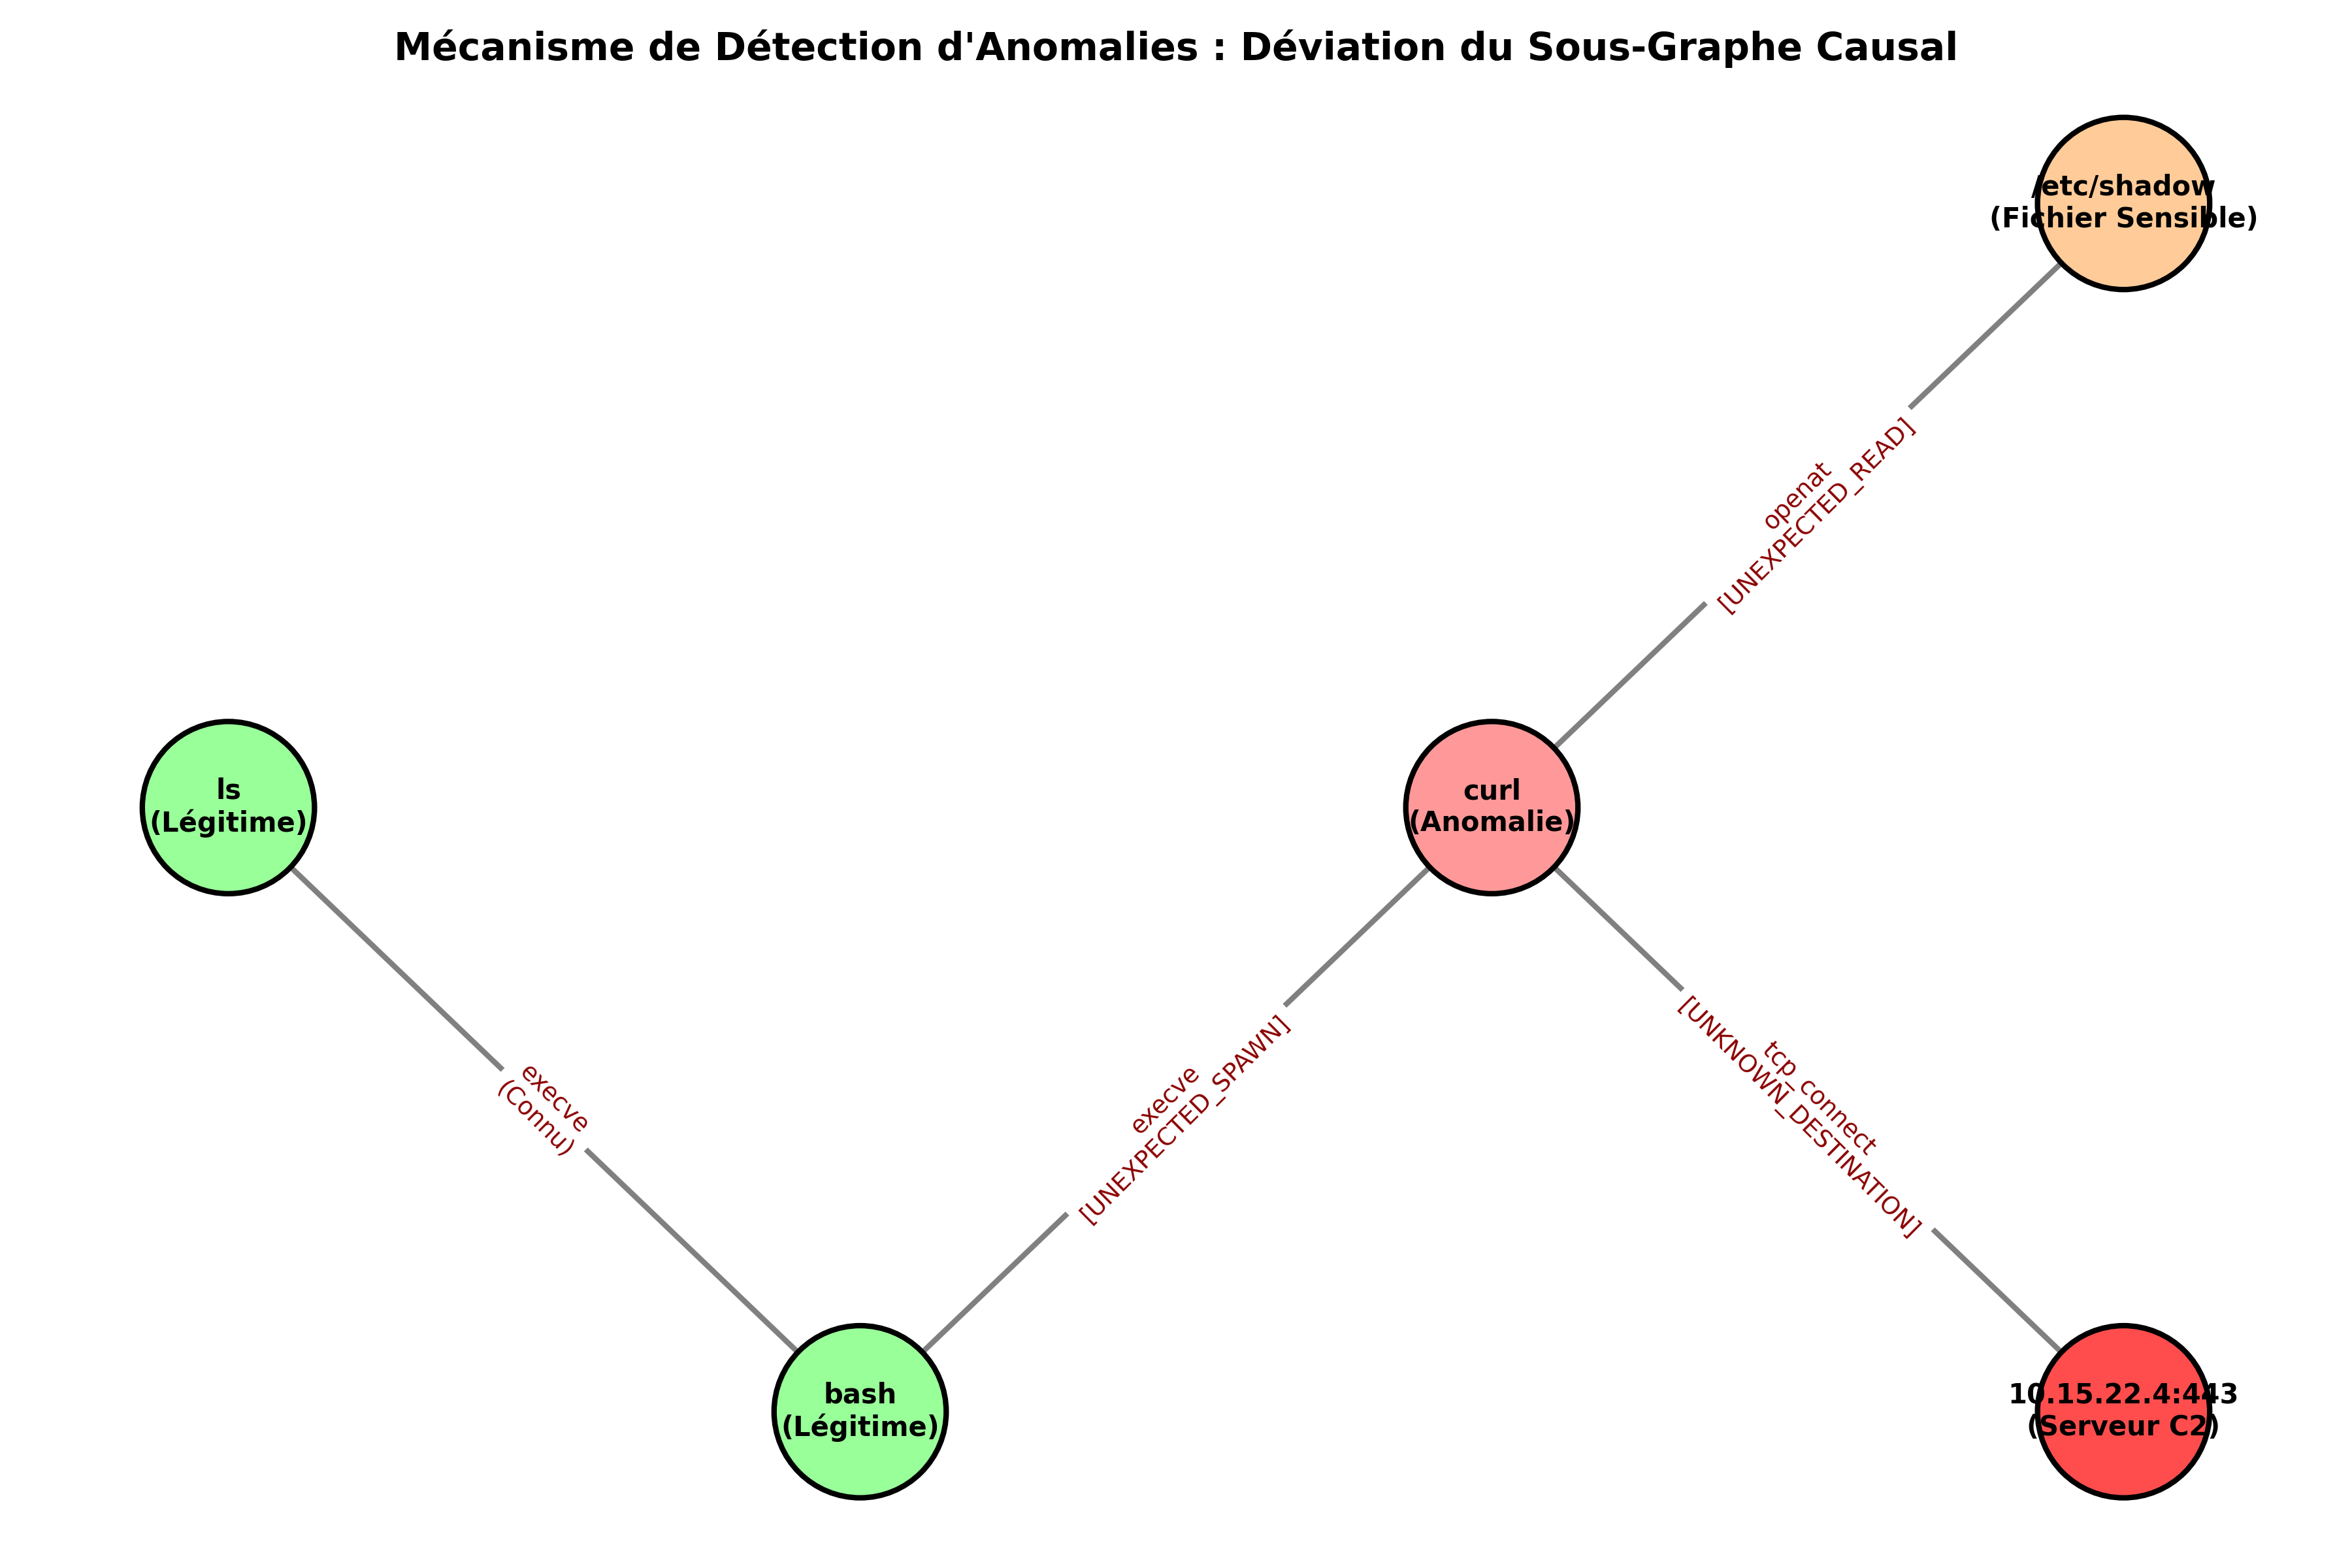
\includegraphics[width=0.9\textwidth]{images/threat_detection_graph.png}
\caption{Schéma conceptuel de la topologie de détection : en vert le sous-graphe modélisant la Baseline attendue, en rouge la déviation structurelle levée par l'exécution malveillante d'un outil ouvrant une exfiltration réseau}
\label{fig:threat_graph}
\end{figure}

\subsection{Analyse de performance}

Même si ce projet n'a pas vocation à fournir une campagne complète de benchmark industriel, nous avons conservé une visualisation synthétique afin d'illustrer l'intérêt d'un filtrage au plus près du noyau. Cette figure résume l'idée défendue dans le projet : limiter le bruit remonté à l'espace utilisateur et réduire le coût du traitement en aval.

\begin{figure}[htbp]
\centering
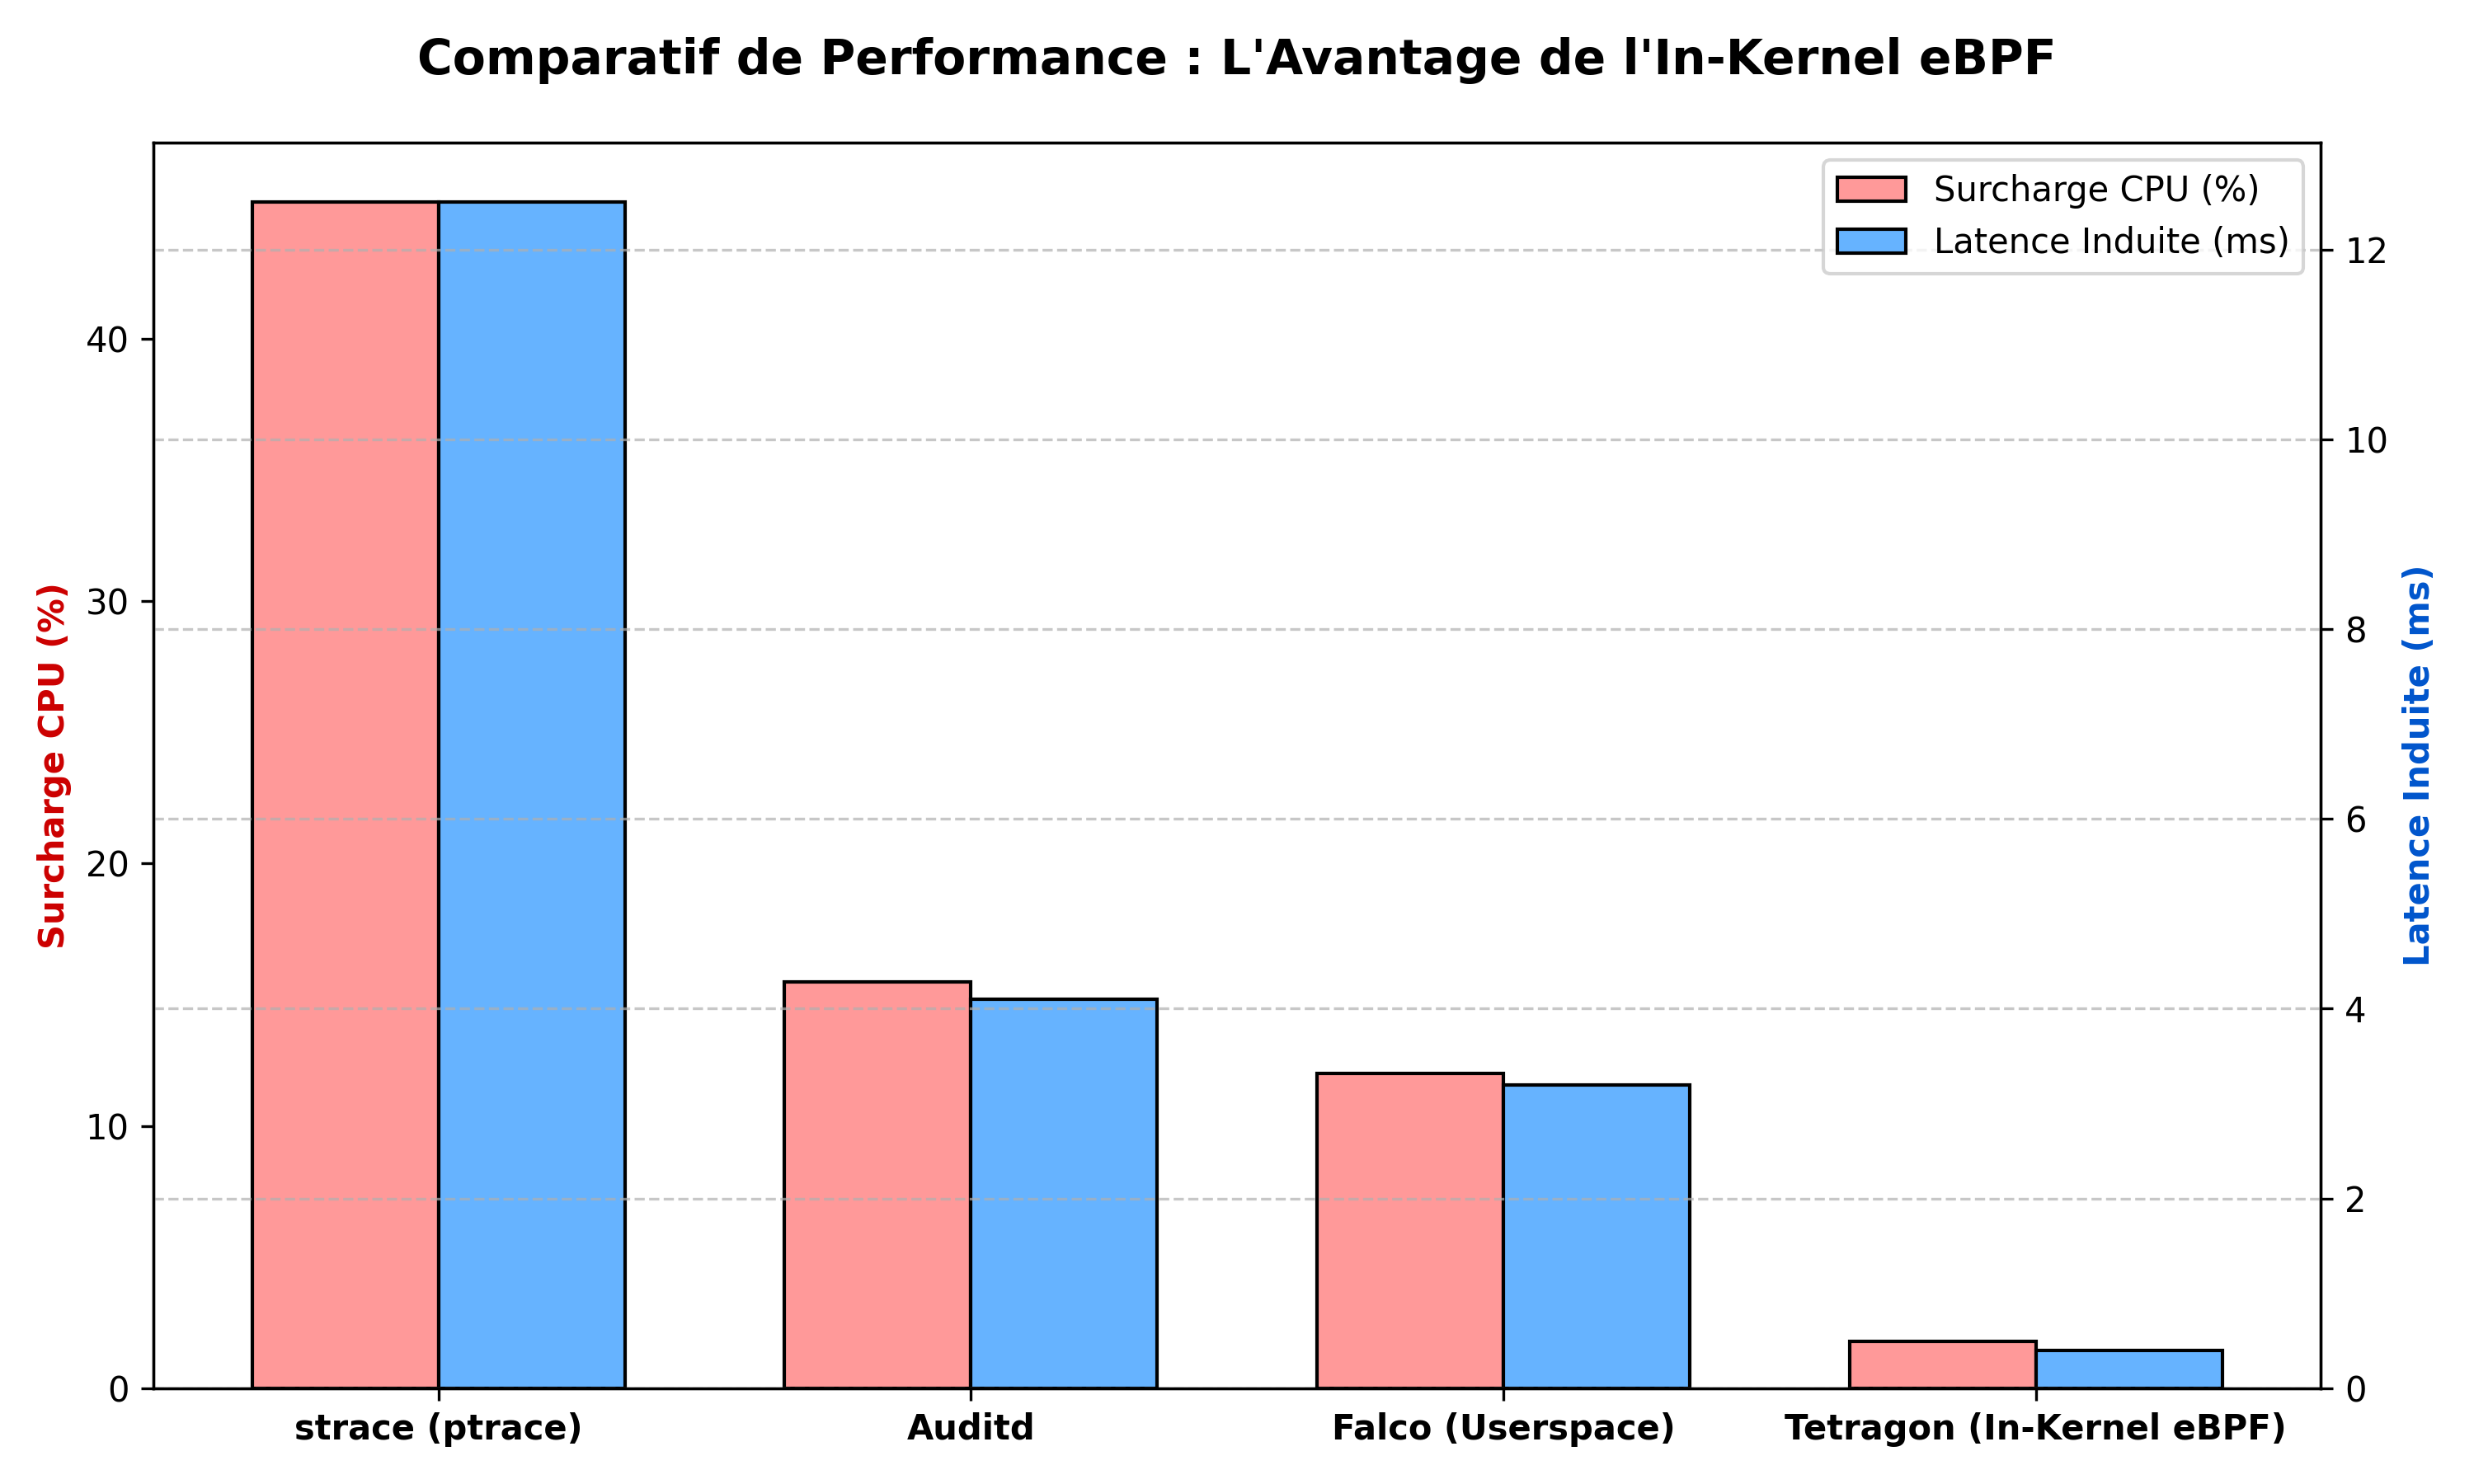
\includegraphics[width=0.9\textwidth]{images/performance_comparison.png}
\caption{Comparaison analytique des performances simulées en termes de charge CPU et de latence induite. L'approche eBPF avec Tetragon vise à réduire les surcoûts en filtrant les événements au plus près du noyau.}
\label{fig:perf_chart}
\end{figure}

\subsection{Visualisation et exploitation opérationnelle}

Le tableau de bord fourni dans \texttt{dashboard/app.py} constitue la partie visible du système. Il est développé avec Streamlit et s'appuie sur des utilitaires de rendu pour transformer le graphe en représentation visuelle. Il permet d'observer un flux d'événements eBPF en direct, de consulter les nœuds et arêtes de façon synthétique et d'afficher les alertes dans une interface exploitable.

Le fonctionnement du dashboard repose sur une logique d'arrière-plan. Lors de l'initialisation, l'application crée un \texttt{EventCollector}, tente de charger une baseline persistée, puis instancie un \texttt{AnomalyDetector}. Un thread daemon est ensuite lancé pour écouter en continu le flux gRPC de Tetragon. Cette conception utilise une synchronisation par verrou afin d'éviter les accès concurrents au graphe et à la liste d'alertes.

Le dashboard expose également des métriques simples, comme le nombre de nœuds, d'arêtes, d'événements traités et d'alertes accumulées. Il propose enfin un mode de test hors ligne par injection de trafic factice, utile pour vérifier l'intégration de bout en bout sans dépendre d'un cluster actif.

\begin{figure}[htbp]
\centering
\includegraphics[width=0.95\textwidth]{images/dashboard_tetragon.png}
\caption{Capture d'écran du Dashboard interactif affichant le graphe causal NetworkX et les anomalies Zero-Day (Tableau latéral)}
\label{fig:dashboard}
\end{figure}

\subsection{Validation fonctionnelle et scénarios offensifs}

La validation du projet a été conduite à deux niveaux complémentaires. Le premier niveau est une validation logicielle classique par tests. Le dépôt contient des tests unitaires dédiés au modèle de graphe, au collecteur, au client gRPC, à l'adaptateur Tetragon, à la baseline et au détecteur. Ces tests vérifient notamment l'extraction des champs critiques, la robustesse face aux événements incomplets, la persistance de la baseline, l'accumulation des comportements observés, la classification des alertes et les niveaux de sévérité associés à certains chemins sensibles. Cette couverture est un élément important du livrable, car elle montre que le projet n'a pas été évalué uniquement par une démonstration visuelle.

Le second niveau de validation est expérimental. Le répertoire \texttt{red\_team/} contient plusieurs scripts destinés à modifier le comportement d'un pod considéré comme légitime pendant la phase d'apprentissage. Le scénario de \textit{reverse shell} simule l'apparition d'un outil réseau inattendu et d'une connexion sortante non cataloguée. Le scénario d'exfiltration combine lecture de fichiers sensibles et émission vers l'extérieur. Un script de \textit{privilege escalation} est également présent dans le dépôt, ce qui montre que le projet a anticipé plusieurs familles d'écarts comportementaux.

L'intérêt de ces scénarios ne réside pas dans leur sophistication offensive, mais dans leur adéquation avec l'objectif de l'IDS. Le système n'a pas besoin de connaître à l'avance le script exact pour réagir ; il suffit que l'exécution introduise un processus non appris, une lecture inhabituelle ou une connexion nouvelle. L'objectif est de montrer la cohérence entre les événements observés, leur modélisation et les alertes remontées.

Il convient toutefois de préciser le périmètre de validation. Le dépôt montre une capacité de détection sur des scénarios contrôlés et sur un environnement localisé. En revanche, il ne fournit pas une évaluation statistique exhaustive sur un cluster de production, ni une mesure complète des performances en charge. Le résultat livré correspond à un prototype expérimental, pas à un produit industriel finalisé.

\subsection{Livraison des éléments demandés}

La livraison finale du projet prend la forme d'un dépôt structuré et exploitable. Les principaux livrables sont les suivants : les manifestes d'infrastructure et politiques Tetragon dans \texttt{infra/}, le code source du pipeline d'ingestion et d'analyse dans \texttt{src/}, le dashboard dans \texttt{dashboard/}, les scénarios d'attaque dans \texttt{red\_team/}, la documentation de prise en main dans le \texttt{README.md}, ainsi que les scripts de lancement \texttt{install.sh} et \texttt{start.sh}. Cette organisation répond directement à l'exigence de livraison d'un système démontrable et non d'une simple description théorique.

Du point de vue académique, la livraison comprend également le rapport, qui documente les hypothèses, les choix techniques, les difficultés rencontrées et les limites observées. Du point de vue technique, le projet est suffisamment empaqueté pour être rejoué : un lecteur peut recréer l'environnement, lancer le flux, ouvrir le dashboard et exécuter les scénarios offensifs. Cette reproductibilité constitue un critère important de qualité, en particulier pour un projet de sécurité où les résultats doivent pouvoir être revérifiés.

En définitive, le projet a permis de réaliser les objectifs principaux : instrumenter un environnement Linux/Kubernetes par eBPF via Tetragon, transformer les événements collectés en graphes comportementaux, apprendre un comportement nominal, détecter des écarts sur cette base et restituer les résultats dans une interface interactive. Les limites restent identifiées, notamment sur l'étendue des scénarios évalués et sur l'absence d'une campagne de performance exhaustive. Le livrable final reste néanmoins cohérent et fonctionnel pour une démonstration académique.

\section{Conclusion}

Ce projet a permis de mettre en place une chaîne complète d'observabilité et de détection fondée sur eBPF, Tetragon et l'analyse de graphes. Le prototype développé montre qu'il est possible de collecter des événements noyau, de les transformer en relations comportementales exploitables, puis de signaler des écarts à partir d'une baseline apprise.

L'approche retenue repose sur des mécanismes simples et explicables : normalisation des événements, construction d'un graphe causal, persistance d'un comportement de référence et comparaison avec les observations courantes. Les essais réalisés sur les scénarios retenus montrent que cette méthode permet de faire remonter plusieurs écarts significatifs sans recourir à des signatures statiques.

Les prolongements possibles concernent l'élargissement des jeux de tests, l'évaluation des performances en charge, ainsi que l'étude de méthodes plus avancées de comparaison de graphes, y compris des approches de type \textit{Graph Neural Networks}.

\newpage
\appendix
\section{Annexes}

Cette section regroupe les principaux éléments techniques venant compléter le rapport principal et démontrant la qualité de réalisation du projet.

\subsection{Arborescence synthétique du projet}

L'organisation du dépôt a été pensée pour séparer clairement l'infrastructure, le moteur d'analyse, l'interface de visualisation, les scénarios offensifs et les tests. L'arborescence utile du projet peut être résumée ainsi :

\begin{lstlisting}[style=annexecode]
Architectural-Blueprint-for-eBPF-Graph-Based-Intrusion-Detection/
├── dashboard/
│   ├── app.py
│   └── utils.py
├── docs/
│   ├── final_Report.tex
│   ├── Rapport-Intermédiaire.tex
│   └── images/
├── infra/
│   ├── k8s/
│   │   └── kind-config.yaml
│   ├── policies/
│   │   ├── trace-exec.yaml
│   │   └── trace-tcp.yaml
│   └── tetragon/
│       └── install.sh
├── red_team/
│   ├── scenario.md
│   └── attacks/
│       ├── exfiltration.sh
│       ├── priv_escalation.sh
│       └── reverse_shell.sh
├── src/
│   ├── analysis/
│   │   ├── baseline.py
│   │   ├── detector.py
│   │   └── storage/
│   └── ingestion/
│       ├── collector.py
│       ├── graph_model.py
│       ├── grpc_client.py
│       ├── tetragon_adapter.py
│       └── proto/
├── tests/
│   ├── test_baseline.py
│   ├── test_collector.py
│   ├── test_detector.py
│   ├── test_graph_model.py
│   ├── test_grpc_client.py
│   ├── test_integration.py
│   └── test_tetragon_adapter.py
├── README.md
└── start.sh
\end{lstlisting}

\subsection{Extrait de code : adaptation des événements Tetragon}

L'un des points importants du projet est la conversion des événements bruts Tetragon vers un format interne plus simple. L'extrait ci-dessous montre le mécanisme de récupération du PID, y compris le repli sur \texttt{execId} lorsqu'il faut décoder un identifiant encodé en Base64.

\begin{lstlisting}[style=annexecode,language=Python]
import base64

def _get_pid_fallback(process_dict: dict, exec_id_key: str = "execId") -> Optional[int]:
    if not process_dict:
        return None
    pid = process_dict.get("pid")
    if isinstance(pid, dict):
        pid = pid.get("value")
    if pid is not None:
        try:
            return int(pid)
        except (ValueError, TypeError):
            pass
    exec_id = process_dict.get(exec_id_key)
    if exec_id:
        try:
            return int(base64.b64decode(exec_id).decode('utf-8').split(':')[-1])
        except Exception:
            pass
    return None
\end{lstlisting}

Ce code évite de perdre certains événements lorsque le PID n'est pas directement fourni sous la forme attendue.

\subsection{Extraits de composants développés}

Les livrables logiciels les plus représentatifs du projet sont organisés autour de plusieurs briques complémentaires :
\begin{itemize}
    \item le pipeline d'adaptation et de normalisation des événements Tetragon, chargé de rendre les flux exploitables par les composants applicatifs ;
    \item le moteur de graphes comportementaux, responsable de la création des nœuds, des arêtes et de la persistance de la baseline ;
    \item le tableau de bord interactif, utilisé pour la visualisation en direct des graphes et des anomalies détectées ;
    \item la suite de scripts offensifs de validation, utilisée pour simuler les scénarios d'attaque retenus dans le cadre des essais.
\end{itemize}

\subsection{Extrait de code : logique de détection d'anomalies}

Le détecteur compare les comportements observés avec ceux qui ont été appris pendant la phase de baseline. L'extrait suivant illustre le cas des connexions réseau inattendues.

\begin{lstlisting}[style=annexecode,language=Python]
elif relation == REL_CONNECTS_TO:
    attrs = tgt_node.get("attributes", {})
    ip = attrs.get("ip", "")
    port = attrs.get("port", "")
    ip_port = "{0}:{1}".format(ip, port)
    if ip_port not in comm_behavior.get("connects", []):
        new_alerts.append(_new_alert(
            severity="HIGH",
            alert_type=ALERT_UNEXPECTED_CONNECTION,
            comm=comm,
            description=(
                "'{0}' connected to '{1}', which was not observed during baseline.".format(
                    comm, ip_port
                )
            ),
            evidence=evidence,
        ))
\end{lstlisting}

Cette logique traduit directement l'idée centrale du projet : un écart comportemental observable dans le graphe doit remonter sous forme d'alerte exploitable.

\subsection{Extrait de code : écoute continue côté dashboard}

Le tableau de bord ne se contente pas d'afficher des données statiques. Il maintient un thread d'écoute qui consomme le flux gRPC de Tetragon en continu.

\begin{lstlisting}[style=annexecode,language=Python]
def grpc_listener(clctr):
    grpc_addr = os.getenv("TETRAGON_GRPC_ADDRESS", "localhost:54321")
    while True:
        try:
            clctr.process_grpc_stream(address=grpc_addr)
        except Exception as e:
            pass
        time.sleep(5)

thread = threading.Thread(target=grpc_listener, args=(local_collector,), daemon=True)
thread.start()
\end{lstlisting}

Cet extrait met en évidence le choix d'une interface temps réel simple à démontrer, sans devoir redémarrer manuellement l'application à chaque nouvel événement.

\subsection{Éléments de reproductibilité}

La reproductibilité du prototype repose sur les éléments suivants :
\begin{itemize}
    \item les scripts d'installation et de configuration du projet ;
    \item les fichiers de déploiement de l'infrastructure locale et du cluster de test ;
    \item les politiques Tetragon utilisées pour la collecte des événements ;
    \item les jeux de tests permettant de rejouer les scénarios légitimes et offensifs décrits dans le compte rendu.
\end{itemize}

\subsection{Exemple de politiques de traçage utilisées}

Le projet s'appuie sur des politiques Tetragon simples afin de capturer des événements lisibles et pertinents. Les exemples ci-dessous montrent les deux points d'entrée utilisés dans le prototype.

\begin{lstlisting}[style=annexecode]
apiVersion: cilium.io/v1alpha1
kind: TracingPolicy
metadata:
  name: "trace-execve"
spec:
  kprobes:
  - call: "sys_execve"
    syscall: true
\end{lstlisting}

\begin{lstlisting}[style=annexecode]
apiVersion: cilium.io/v1alpha1
kind: TracingPolicy
metadata:
  name: "trace-tcp-connect"
spec:
  kprobes:
  - call: "tcp_connect"
    syscall: false
\end{lstlisting}

Ces politiques sont suffisantes pour produire une base d'observation utile sur les lancements de processus et les connexions sortantes.

\subsection{Scripts de lancement et de démonstration}

Deux scripts participent directement à la prise en main du projet :
\begin{itemize}
    \item \texttt{infra/tetragon/install.sh} automatise la création du cluster Kind, l'installation de Tetragon et l'application des politiques ;
    \item \texttt{start.sh} lance le \textit{port-forward} gRPC puis démarre le dashboard Streamlit.
\end{itemize}

À cela s'ajoutent les scripts du répertoire \texttt{red\_team/attacks/}, utilisés pour rejouer les scénarios de validation offensifs dans le cluster.

\newpage
\begin{thebibliography}{9}

\bibitem{tetragon_web}
Projet Tetragon. \textit{eBPF-based Security Observability and Runtime Enforcement}. Disponible sur : \url{https://tetragon.io/} (Consulté en 2025).

\bibitem{cilium_web}
Projet Cilium. \textit{eBPF-based Networking, Observability, Security}. Disponible sur : \url{https://cilium.io/} (Consulté en 2025).

\bibitem{ghane2025observability}
Ghane, Dr Mehdi. \textit{Observability Engineering Fundamentals}. In : Observability Engineering with Cilium: Observability Magic in the Cloud-Native Journey with Hubble and Tetragon. Berkeley, CA: Apress, Springer, 2025. p. 83-147.

\bibitem{scholz2018performance}
Scholz, Dominik, et al. \textit{Performance implications of packet filtering with linux ebpf}. In : 2018 30th International Teletraffic Congress (ITC 30). Vol. 1. IEEE, 2018.

\bibitem{vieira2020fast}
Vieira, Marcos AM, et al. \textit{Fast packet processing with ebpf and xdp: Concepts, code, challenges, and applications}. ACM Computing Surveys (CSUR) 53.1 (2020): 1-36.

\bibitem{gbadamosi2024ebpf}
Gbadamosi, Bolaji, et al. \textit{The eBPF runtime in the linux kernel}. arXiv preprint arXiv:2410.00026 (2024).

\end{thebibliography}

\label{fin}
\end{document}
